\begin{figure}
\begin{center}
    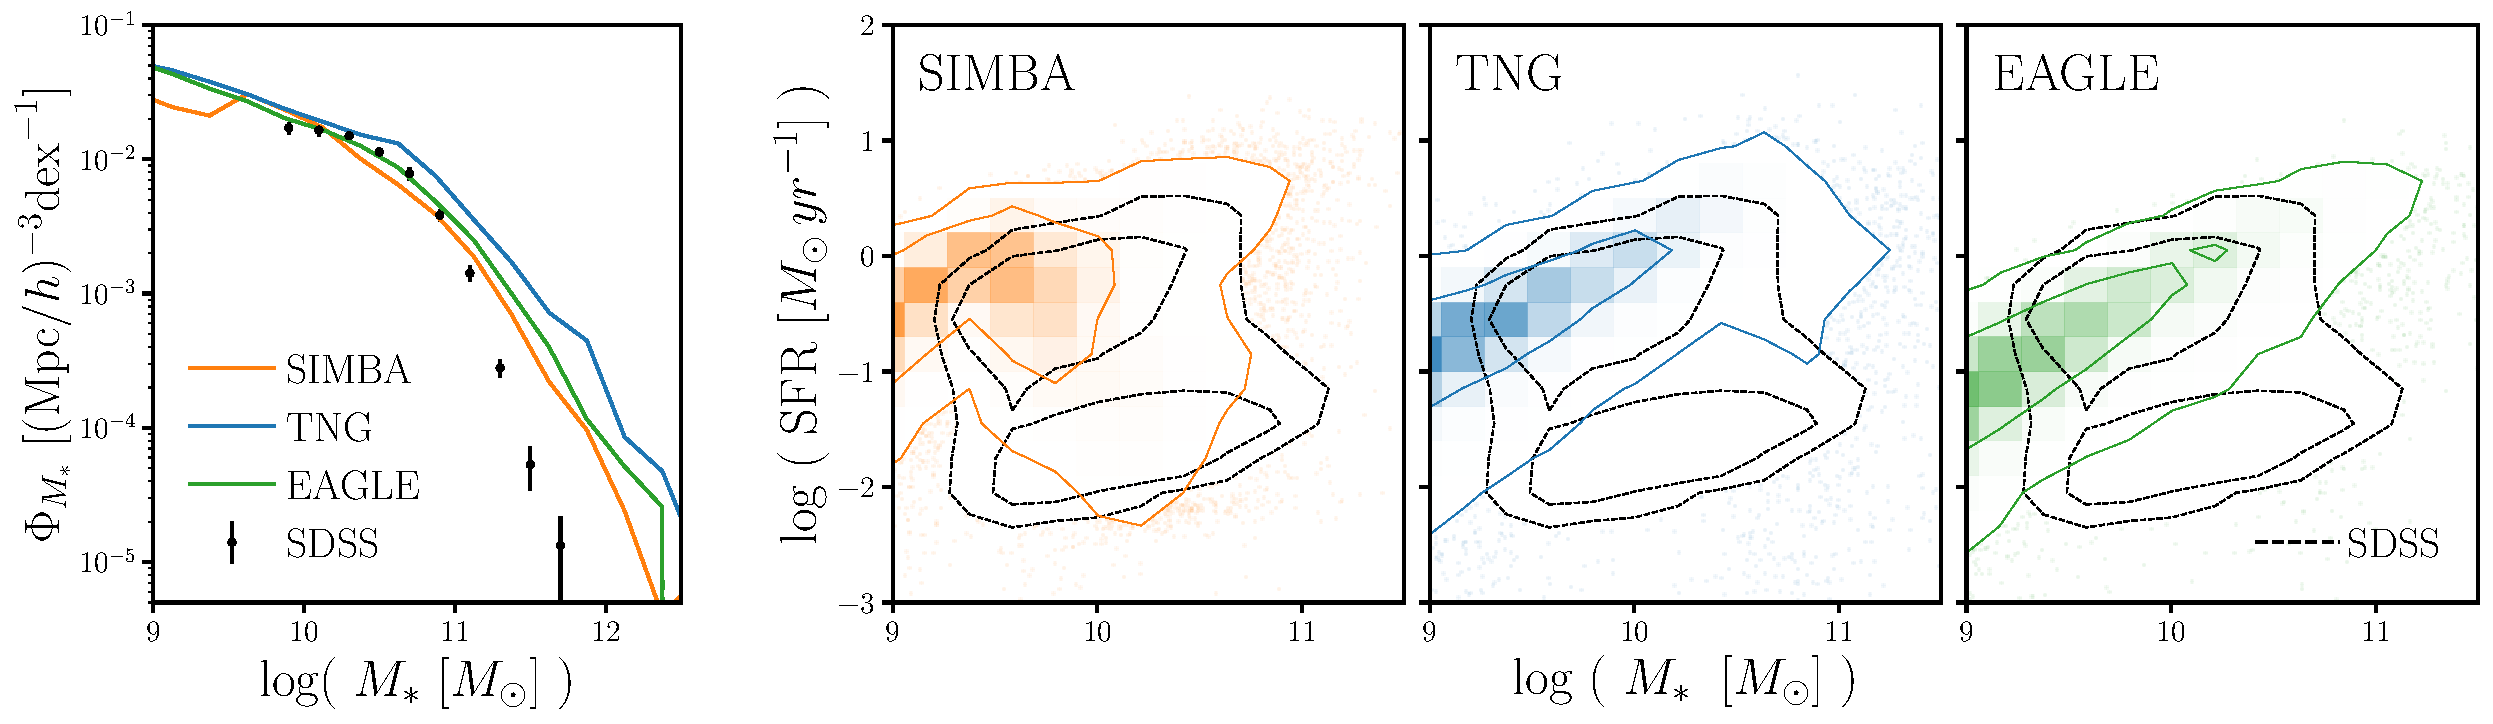
\includegraphics[width=\textwidth]{figs/smf_m_sfr.pdf}
    \caption{\label{fig:smf_msfr}
    The stellar mass functions ($\Phi_{M_*}$; left-most panel) and $M_*-\sfr$
    relation (right panels) of simulated galaxies from SIMBA (orange), TNG
    (blue), and EAGLE (green). For reference, we include $\Phi_{M_*}$ (black)
    and the $M_*-\sfr$ relation (black dashed) of our SDSS galaxy sample. 
    Uncertainties for the SDSS $\Phi_{M_*}$ are derived using jackknife resampling. 
    In Section~\ref{sec:sims}, we describe the simulations and observations above.
    Differences in $\Phi_{M_*}$ and the $M_*-\sfr$ relations among the
    simulations highlight that the \emph{hydrodynamical simulations predict
    galaxy populations with significantly different the physical properties.} 
    }
\end{center}
\end{figure}

\section{Data}\label{sec:sims}
In this paper we apply empirical dust attenuation (\eda) prescriptions to galaxies 
in the Illustris TNG, EAGLE, and SIMBA cosmological hydrodynamical simulations. 
For each galaxy in the \eda output, we forward model the spectral energy distributions 
(SED) and measure the $r$-band luminosity ($M_r$), optical color ($G-R$), and
UV color ($FUV-NUV$) from the SEDs. These forward modeled observables, unlike
physical properties such as $M_*$ and $\sfr$, are \emph{consistently} defined
and derived in both simulations and observations. Afterwards, we compare the
predicted \eda observables to galaxies in the SDSS observations. Below, we
briefly describe the hydrodynamical simulations and the SDSS observations used
throughout this work.

In Figure~\ref{fig:smf_msfr}, we present the stellar mass functions
($\Phi_{M_*}$; left-most panel) and $M_*-\sfr$ relations (right panels) for
simulated galaxies of SIMBA (orange), TNG (blue), and EAGLE (green). 
We include, for reference, $\Phi_{M_*}$ and the $M_*-\sfr$ relation for
our SDSS galaxy sample. The uncertainties for the SDSS SMF are derived 
from jackknife resampling. For the simulations, $M_*$ is the total stellar mass 
within the host halo, excluding any stellar mass in subhalos; $\sfr$ is the
instantaneous $\sfr$ derived from dense and cold gas. For SDSS, $M_*$ is
estimated using $\mathtt{kcorrect}$~\citep{blanton2007a} 
assuming a~\cite{chabrier2003} initial mass function and $\sfr$ are from the
current release of
\cite{brinchmann2004}\footnote{\url{http://www.mpa-garching.mpg.de/SDSS/DR7/}}.
%We describe the simulations and observations furthers in sections below. 
Figure~\ref{fig:smf_msfr} illustrates that the hydrodynamical simulations
predict significantly different SMFs and $M_*-\sfr$ relations. 
This difference, which was also recently highlighted in \cite{hahn2019c}, 
demonstrates that \emph{the hydrodynamical simulations predict galaxy
populations with significantly different physical properties}.

\subsection{Illustris TNG} \label{sec:tng}
The Illustris TNG simulation\footnote{\url{https://www.tng-project.org/}}
(hereafter TNG) is a cosmological hydrodynamical simulation of comoving 
volume $(110.7\,\mpc)^3$~\citep{nelson2018, pillepich2018, springel2018}. It
improves on the original Illustris
simulation\footnote{\url{http://www.illustris-project.org}}~(\citealt{vogelsberger2014, genel2014};
public data release by~\citealt{nelson2015}), by including
magneto-hydrodynamics and updated treatments for galactic winds, metal
enrichment, and AGN feedback. Most notably, TNG uses a new implementation for
feedback from SMBH~\citep{weinberger2018}, where feedback energy is injected in
the form of a kinetic AGN-driven wind at low SMBH accretion rates. This new
implementation has been shown to alleviate discrepancies found between the
original Illustris and observations for $> 10^{13-14} M_\odot$ massive halos. 
%TNG has a baryonic mass resolution of $1.4\times10^6M_{\sun}$ \ch{temporal resolution?}.
\todo{details on the following properties that we use in the paper: SFH, ZH}

\subsection{EAGLE} \label{sec:eagle} 
We use L0100Ref of the Virgo Consortium's EAGLE
project\footnote{\url{http://www.eaglesim.org}}, a publicly available suite of
cosmological hydrodynamic simulations~\citep{schaye2015, crain2015,
mcalpine2016}. The simulation has a comoving volume of $(100\,\mpc)^3$ and % baryonic mass resolution of $1.81\times 10^6M_{\sun}$. It 
is simulated with the {\sc Anarchy} code (Dalla Vecchia et al. in prep.; 
see also Appendix A of \citealt{schaye2015}), a modified version of the 
{\sc GADGET-3} code~\citep{springel2005}.
%that includes a conservative pressure-entropy formulation for the smoothed particle hydrodynamics calculation, artificial viscosity, artificial conduction and the time limiter that improve hydrodynamic computation performance. 
It has subgrid models for star formation, stellar mass loss, metal enrichment
and stellar feedback that stochastically inject thermal energy in the ISM as
in~\citep{dallavecchia2012}; the feedback energy from AGN is also added to
surrounding gas stochastically~\citep{booth2009}. Parameters of the stellar 
feedback and SMBH accretion are calibrated to broadly reproduce the $z=0$ 
stellar mass function and galaxy stellar size-stellar mass relation. Meanwhile, 
the AGN feedback efficiency is calibrated to match the SMBH-galaxy mass relation. 
\todo{details on the following properties that we use in the paper: SFH, ZH}

\subsection{SIMBA} \label{sec:simba}
The {\sc Simba} simulation suite~\citep{dave2019}, the successor to {\sc
Mufasa}~\citep{dave2016, dave2017, dave2017a}, is a cosmological hydrodynamical
simulation construted using {\sc Gizmo}, a meshless finite mass hydrodynamics 
code~\citep{hopkins2015, hopkins2017}. Of the simulations, we use
`m100n1024', which has a box size of $(100\,h^{-1}\,\mpc)^3$ and baryonic 
mass resolution of $1.82 \times 10^7\ M_\odot$. The simulation uses the same
subgrid models as {\sc Mufasa} for $\rm H_2$ based star formation, decoupled
two-phase winds for star formation driven galactic winds, and feedback from 
Type I supernovae and AGB stars. Meanwhile, it uses updated models for AGN
feedback and on-the-fly dust model. {\sc Simba} uses a two-mode SMBH accretion 
model, torque-limited accretion for cold gas~\citep{angles-alcazar2017} and 
Bondi-based accretion for hot gas, and two-mode AGN feedback. %which ejects bipolar kinetic winds with $\sim 10^3 \kms$ for high SMBH accretion rate, and launches winds with increased velocity of $\sim 8000 \kms$ for low SMBH accretion of Eddington ratio below 2 \%.
\todo{details on the following properties that we use in the paper: SFH, ZH}

\subsection{Forward Modeled Spectral Energy Distributions} \label{sec:fm} 
\todo{describe how the SED is generated using the SFH and ZHs} 

In Figure~\ref{fig:obs} we present the optical and UV color-magnitude
relations, $(\gr)-M_r$ (top) and $(\fnuv)-M_r$ (bottom), for central galaxies
of the SIMBA (left), TNG (center) and EAGLE (right) simulations. The $\gr$ and
$\fnuv$ colors are derived from the forward modeled SED and absolute magnitudes.
The observables for the simulations do not yet include any prescription for dust
attenuation. Comparison to SDSS centrals (black dashed) clearly demonstrate
that {\em without dust attenuation, the hydrodynamical simulations cannot
reproduce the observed optical or UV color-magnitude relations.}

\subsection{SDSS Galaxies} \label{sec:obs} 
The \eda model provides a flexible prescription for assigning dust attenuation
to simulated galaxies so that the hydrodynamical simulations, described above,
can reproduce observations. Throughout this work, for our observations, we use
a galaxy sample derived from SDSS.  %Throughout this work, we use the \cite{tinker2011} SDSS central galaxy sample as our observation. 
We impose a $M_r < -20$ completeness cut on the \cite{tinker2011} volume-limited 
sample that is complete above $M_* > 10^{9.4} h^{-2}M_\odot$. The original
\cite{tinker2011} sample is derived from the SDSS DR7~\citep{abazajian2009} NYU
Value-Added Galaxy Catalog~\citep[VAGC;][]{blanton2005}. In this work, we focus 
on observables that can be consistently defined and derived in both simulations 
and observables: $M_r$, $\gr$, and $\fnuv$. For our SDSS sample, we use $FUV$,
$NUV$, $r$ and $g$ band absolute magnitudes from the NASA-Sloan
Atlas\footnote{\url{http://nsatlas.org/}}. These absolute magnitudes are
derived using $\mathtt{kcorrect}$~\citep{blanton2007a}, assuming
a~\cite{chabrier2003} initial mass function, and use SDSS photometry with
improved background subtraction~\citep{blanton2011}. 

\begin{figure}
\begin{center}
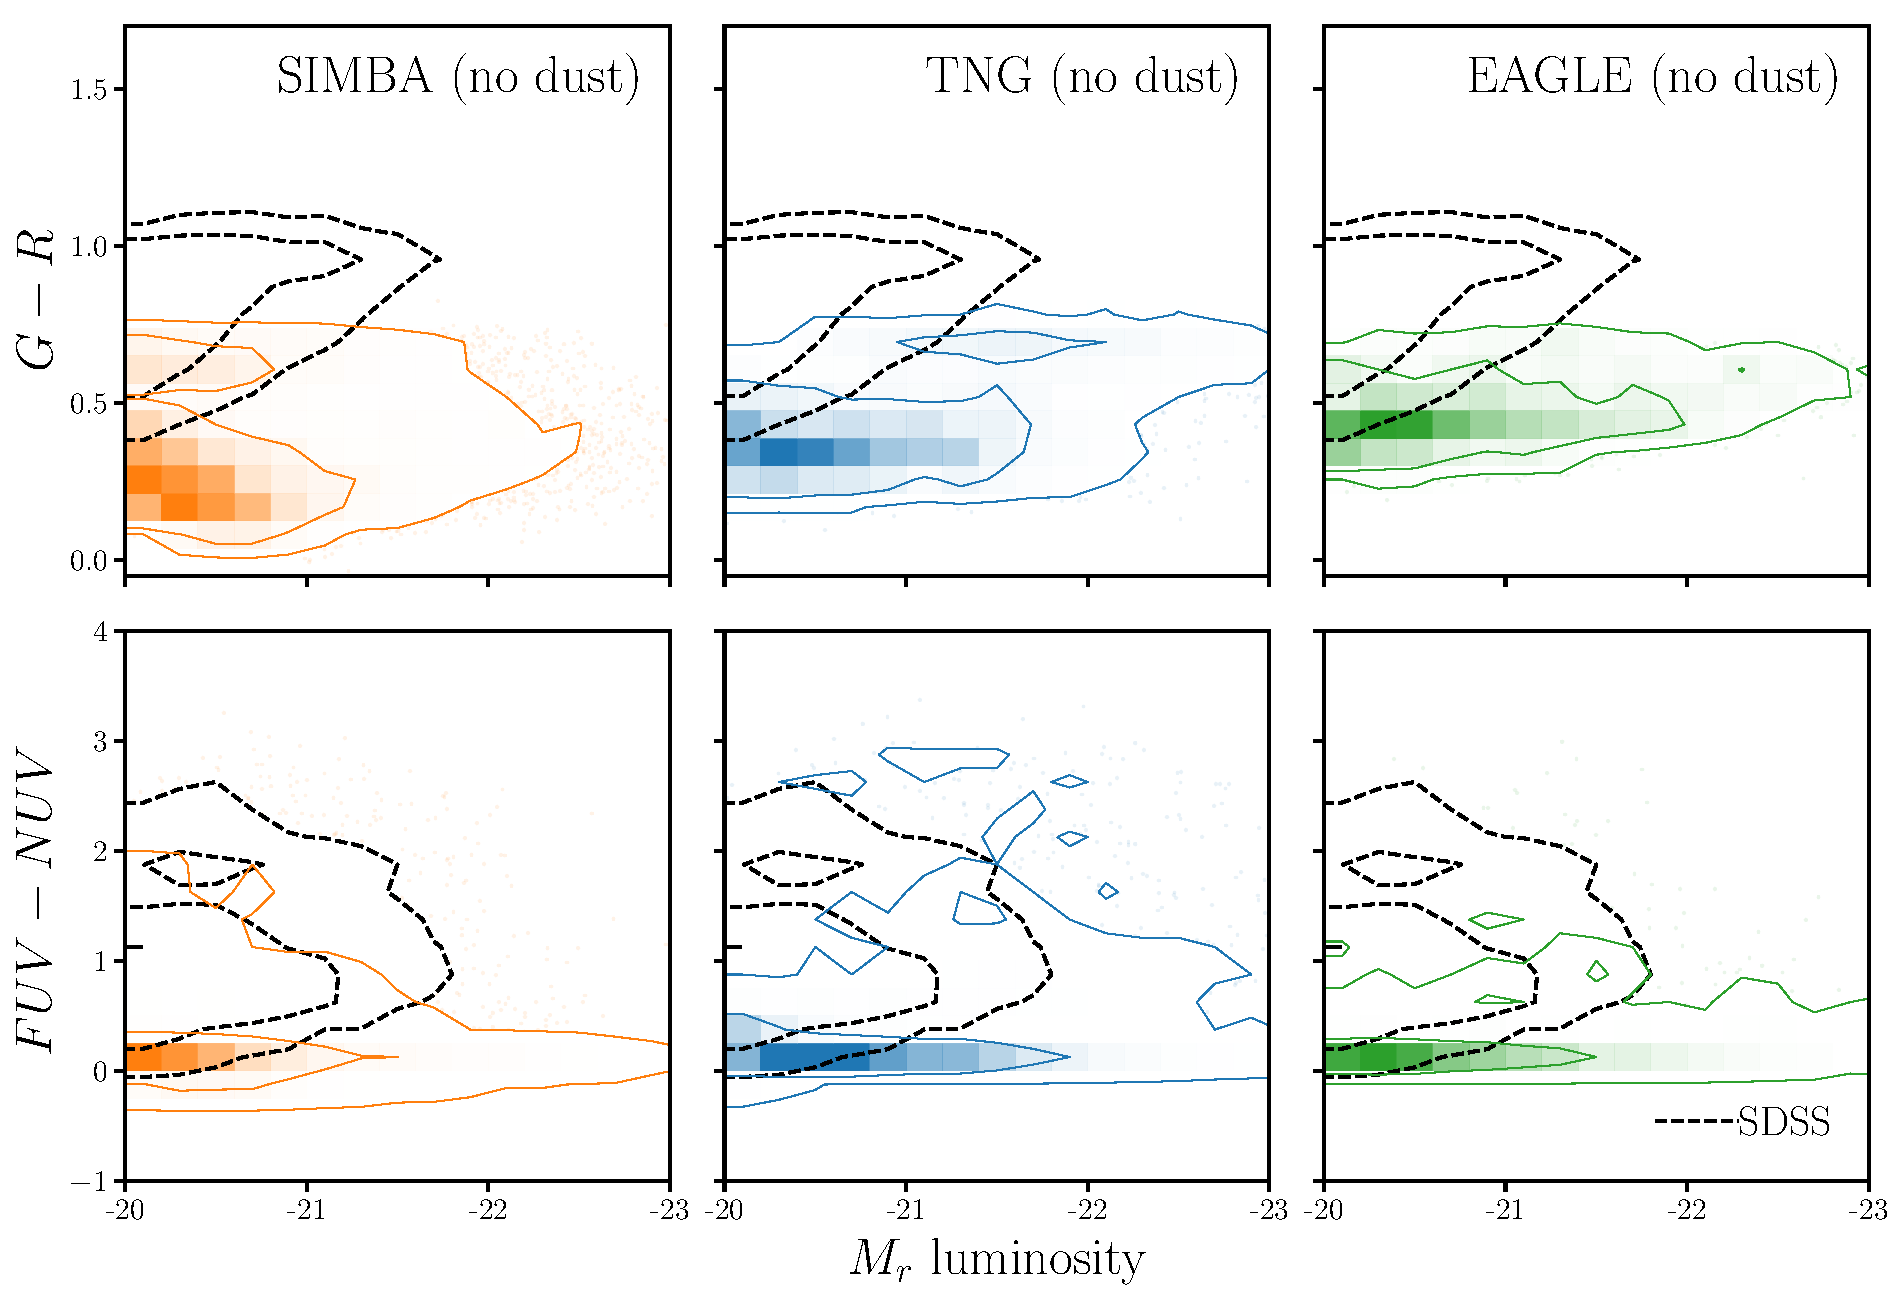
\includegraphics[width=0.9\textwidth]{figs/observables.pdf} 
    \caption{\label{fig:obs}
    We present the optical and UV color-magnitude relations of simulated galaxies
    in SIMBA (left), TNG (center), and EAGLE (right). The simulations above do 
    {\em not} yet include the \eda or any prescription for dust attenuation. 
    $(\gr)-M_r$ (top) and $(\fnuv)-M_r$ (bottom) are the main observables used 
    throughout the paper. They are derived from forward modeled SEDs and, thus, 
    are consistently defined and measured as SDSS observations
    (Section~\ref{sec:fm}). For comparison, we include the distributions of our
    SDSS sample (black dashed). {\em Without dust, the hydrodynamical simulations 
    cannot reproduce the observed optical or UV color-magnitude.}
    }
\end{center}
\end{figure}
